Bitcoin mining, as already anticipated, is a mechanism which constitutes a foundational piece of the entire protocol. To put it simply, <<mining is a lottery to create new blocks in the Bitcoin blockchain. There are two main purposes for mining:
\begin{enumerate}
    \item To Permanently add transactions to the blockchain without the permission of any entity.
    \item To fairly distribute the 21 million bitcoin supply by rewarding new coins to miners who spend real world resources (electricity) to secure the network.>> \cite{bitcoinmininghandbook}
\end{enumerate} 

\noindent In order to mine a valid block, miners need to find the pre-image which corresponds to a \textit{hash} (or \textit{digest}) which satisfies the current Bitcoin network difficulty. As described earlier, the difficulty adjustment mechanism regulates the mining difficulty for the entire Bitcoin network, every 2016 blocks. From a practical point of view, what it does is to simply increase or decrease a value which is present into Bitcoin block headers, which is called \textit{\textbf{target}} (or \textit{nBits}). The \textit{target} represents the current maximum value that a hash found by miners has to be, in order to be considered valid for the entire network. From another point of view, it represents the size of the set of valid solutions for the current PoW algorithm.\\
\noindent Of course, the object which miners utilize as input for the SHA-256 hash function, is a block fulfilled with transactions received from their Bitcoin full-nodes. More specifically, the input is constituted by the \textbf{block header} which is derived from the block template built by miners, along with a random value called \textbf{nonce}. The \textit{nonce} is constantly changed until a valid hash value is found.\\
As represented in \ref{fig:block_header_fields}, miners build the so-called \textit{candidate block}, which contains all the best transactions received from their full-nodes (which typically are the transactions that pays more fees to be firstly included in a new block). Once they got the transactions, they need to complete the \textit{candidate block} by building the corresponding block header, which includes the following fields:
\begin{itemize}
    \item \textbf{Version}: a 4 bytes field which indicates the version of the Bitcoin protocol being used. It allows for future upgrades and compatibility with different protocol enhancements.
    \item \textbf{Previous Block Hash}: a 32 bytes field  which contains the hash value of the previous block in the blockchain. It links the current block to the previous one, forming a chain of blocks.
    \item \textbf{Merkle root}: a 32 bytes hash computed by combining the transaction hashes of all the transactions included in a particular block. These transaction hashes are then paired and hashed together until a single hash is obtained.
    \item \textbf{Difficulty target}: a 4 bytes field that represents the current network difficulty level, which, as already explained, indicates the maximum allowed value for the block hash to be considered valid.
    \item \textbf{Timestamp}: a 4 bytes field that records the approximate time when the block was mined. 
    \item \textbf{Nonce}: a 32-bit value that miners adjust in their attempts to find a valid block hash. Miners repeatedly change the nonce, double hash the block header, and check if the resulting hash meets the difficulty requirement.
\end{itemize}
\begin{figure}[h!]
\centering
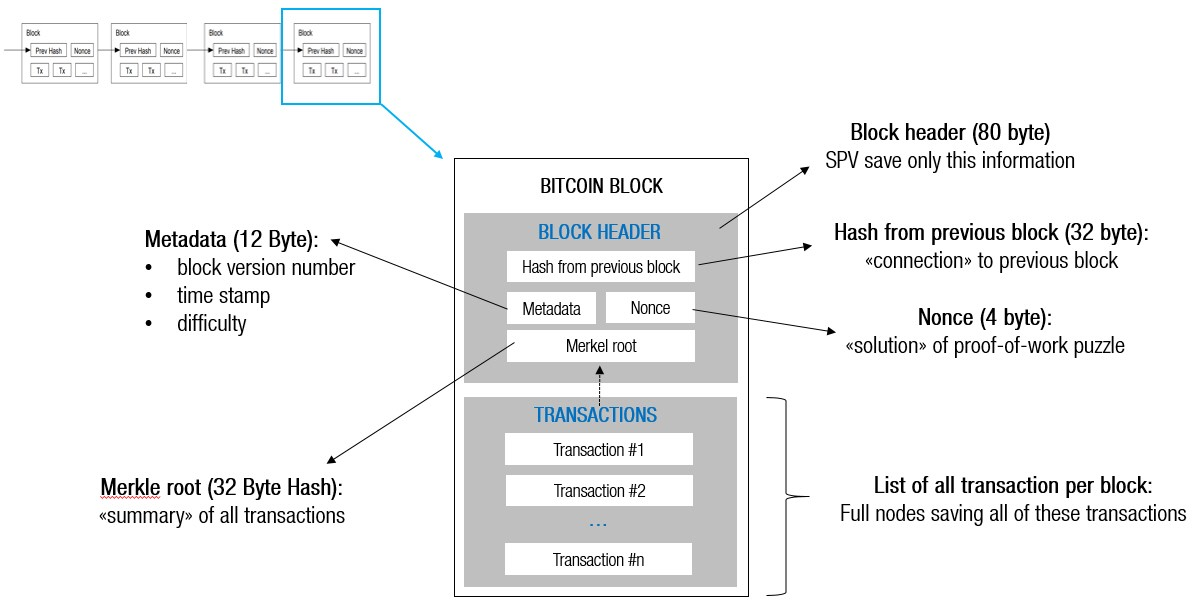
\includegraphics[width=15cm]{Figures/mining/bitcoin-block-header.jpeg}
\caption{Bitcoin block and block header fields}
\label{fig:block_header_fields}
\end{figure}

\begin{wrapfigure}{r}{0.6\textwidth}
\centering
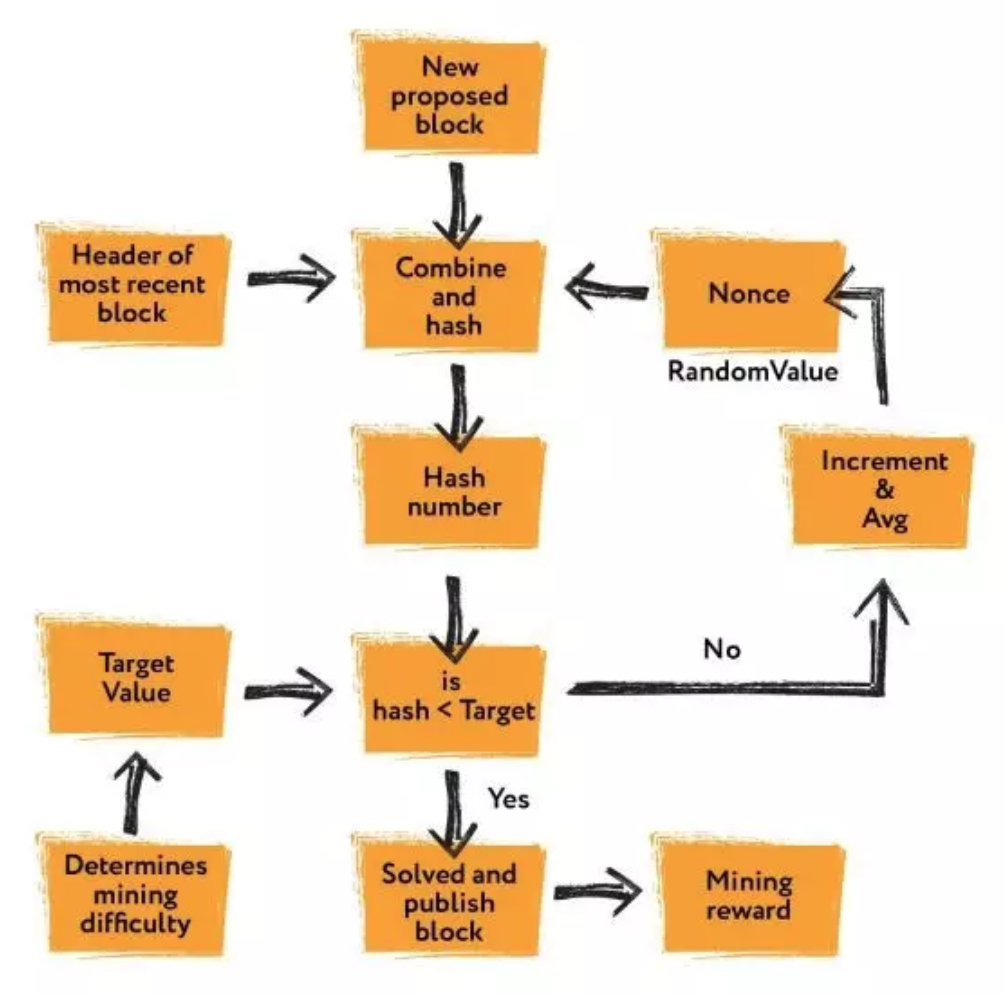
\includegraphics[width=0.55\textwidth]{Figures/mining/mining-flow-chart.png}
\caption{Flow chart of mining activity}
\label{fig:mining-flow-chart}
\end{wrapfigure}
Basically, during mining activity, the miner tries to solve the Proof-of-Work by constantly changing the nonce value contained in the block header which is working on. Every time the miner applies a \textbf{double SHA-256} to the block header, and if the output is greater than the current Bitcoin difficulty \textit{target}, the miner needs to increment the nonce value and retry the double hash again.
When the output of the double SHA-256 corresponds to a number which is less than the Bitcoin current target, it means the miner found a valid solution to the Proof-of-Work, and so he adds the new mined block to its local copy of the blockchain and he immediately broadcasts the new block to all the other peers which he is connected to. He needs to be as fast as possible during the so-called \textit{block-propagation}, since it's crucial to let him claim the \textbf{\textit{block reward}}.
To better resume the mining activity, the flow chart present in Figure \ref{fig:mining-flow-chart} can be very helpful.\\

\noindent In the Bitcoin ecosystem, miners play a crucial role by utilizing electricity to solve the above-described Proof-of-Work. When a miner successfully completes the task and validates all the transactions according to the consensus rules, they become eligible to receive a reward. This reward is typically in the form of new minted Bitcoin and transaction fees. Importantly, the reward is granted only when the miner demonstrates their ability to accurately validate the transactions without the need for a central authority. This delicate balance between mining, validation, and reward ensures the security of Bitcoin's network.\\\\
As already anticipated, the reward is constituted by the sum of the block reward and transaction fees from all the transactions included in the block. This quantity is contained and encoded in the so-called \textbf{\textit{coinbase transaction}}. Differently from regular transactions in Bitcoin, the coinbase transaction does not use Unspent Transaction Outputs (UTXOs) as inputs. Instead, it contains only one input known as the coinbase, which essentially generates new Bitcoin out of nothing. The coinbase transaction has a single output, which is designed to be paid to the miner's own Bitcoin address.
